\documentclass[a4paper]{report}

% This Template was kindly provided by Inna Pirina
% Special thanks to Christopher Dilley for providing the formulas

% do not ignore non-ascii chars
\usepackage{fontspec}
\usepackage[top=2cm]{geometry}
% use harvard-style referencing
\usepackage[round]{natbib}
\renewcommand{\bibname}{References}
\bibliographystyle{abbrvnat}
% needed for URLs
\usepackage[hidelinks]{hyperref}
% beautiful tables
\usepackage{booktabs}
% set the font size of captions
\usepackage[font=small]{caption}
\usepackage{blindtext}
\usepackage{graphicx}
\usepackage{amsmath}
\usepackage{multirow}

\begin{document}

\title{Optimized computational modeling of adaptive activation-based concept learning}
\bigskip
\author{
	Velislav Slavov \\ \normalsize{author} \\ \normalsize\url{velislav.slavov@student.uni-tuebingen.de}\medskip
	\and
	Dr. Detmar Meurers \\ \normalsize{advisor} \\ \normalsize\url{dm@sfs.uni-tuebingen.de}\bigskip
}
\date{September 2018}
\maketitle



\begin{abstract}

When faced with the challenges of vocabulary learning, technology has been proven to provide increased results compared to conventional learning methods by implementing explicit formal models of human cognition. One such model was developed by Philip Pavlik and John Anderson and was based on the ACT-R cognitive architecture. Applying algorithm optimization techniques to their algorithm and increasing its computational efficiency promotes its application in real-life learning systems. This thesis develops an implementation of the Pavlik and Anderson model which should improve its efficiency without sacrificing effectiveness in language learning tasks.

\end{abstract}



\section*{Declaration of Authorship}
I hereby declare that this thesis, titled "Optimized computational modeling of adaptive activation-based concept learning", is my own unaided work. All direct or indirect sources used are acknowledged as references.
I am aware that the thesis in digital form can be examined for the use of unauthorized aid and in order to determine whether the thesis as a whole or parts incorporated in it may be deemed as plagiarism. For the comparison of my work with existing sources I agree that it shall be entered in a database where it shall also remain after examination, to enable comparison with future theses submitted. Further rights of reproduction and usage, however, are not granted here.
This paper was not previously presented to another examination board and has not been published.



\chapter{Introduction}
Factual learning is an important part of human development and can be found in every aspect of everyday life. One of the increasingly popular fields, where this process takes place is language learning and in particular - vocabulary learning. While an individual gains knowledge of their mother tongue through a process referred to as "language acquisition" (due to the fact that learning happens mostly passively), learning further languages requires a conscious effort from the learner, in which case it is referred to as "language learning". (\cite{clark09}, \cite{cooksingleton08})

Cognitive psychology has been able to identify a number of patterns, which explain how humans process information, such as the modality effect, the testing effect and the spacing effect. The increasing use of technology to facilitate learning and the development of cognitive architectures such as the Adaptive Control of Thought—Rational (known as ACT-R) provides a real-life application for such patterns and allows educators to develop learning systems, which reliably produce improved results. \citep{anderson18}. One of the challenges of applying such a system in real life is developing an algorithm complex enough to accurately model human cognition as well as one that performs efficiently enough to not hinder the learner's interaction with the system.

The goal of this thesis is to analyze an adaptive activation-based learning model, based on the ACT-R architecture and try to develop a more computationally efficient implementation of that model. The performance as well as the accuracy of the resulting implementation will be compared to the original implementation of the learning model by conducting a series of experiments, which simulate real learning conditions.

In Chapter 1 we will provide a short introduction to ACT-R, the learning model, which is used as a basis for this thesis as well as common algorithm optimization techniques and how they apply to the algorithm at hand. Chapter 2 provides an explanation of the optimization process and Chapter 3 discusses the results of the conducted experiments.


\chapter{Background}
This section introduces the two aspects of the optimization process. First it describes research done in the field of human cognition and introduces the learning algorithm, which serves as the base for optimization, and then describes techniques commonly used to optimize the algorithm given stated challenges.

\section{The spacing and testing effects}
When it comes to factual learning tasks, massed learning (colloquially known as cramming) has become the go-to approach. It consists of exposing the learner to a big amount of information for a short amount of time in an attempt to prepare the learner for an upcoming examination on the studied material. Research, however, has shown that massed learning only produces short-term results and therefore is unsuitable for achieving long-term information retention. The proposed alternative for effective long-term results is the so-called distributed (or spaced) learning, which is based on Ebbinghaus' theory that spacing the individual item interactions \footnote{The pairs "vocabulary item" - "word" and "item interaction" - "word encounter" will be used interchangeably from now on.} further apart actually produces consistent long-term retention. This discovery is known as the "spacing effect". Furthermore, spaced learning attempts to optimize both intra-session intervals (how often each word gets presented within a study session) and inter-session intervals (how far apart individual study sessions should take place). \citep{ebbinghaus85}

\section{The basics of ACT-R}
Since the model, which is being analyzed in this thesis is based on the ACT-R cognitive architecture, we will provide a very superficial introduction to it in order to introduce some important terminology and concepts. ACT-R stands for "Adaptive Character of Thought - Rational" and its aim is to explain and formally define how humans perceive and express both declarative and procedural knowledge. \citep{andbothell04}. Declarative knowledge refers to the ability of the human brain to retrieve \textbf{factual information}, whereas procedural knowledge is connected to the subconscious ability to accomplish somewhat \textbf{complex procedures} (riding a bicycle, going up the stairs, writing a text etc.). Since vocabulary learning can be compared to learning facts, the model described in this thesis will make use of the implementation of declarative memory in the ACT-R architecture. The model is also referred to as an activation-based one, as it relies on the concept of "activations", which ACT-R defines as the strength of each vocabulary item in the learner's memory. \citep{woudenberg08}

\section{The Pavlik and Anderson model}
Pavlik and Anderson have managed to formalize this research into their model by modifying the base ACT-R formula for calculating activations. \citep{panderson05}. An item's activation is expressed as a power function of the sum of the time deltas of its previous encounters (how long ago each encounter occurred), scaled by the rate of decay at the given encounter (how fast the activation decays with the passage of time). This results in the latest encounters having the highest impact on the item's current activation \footnote{The definition of "word encounter" varies depending on the learning system. It could consist of presenting word-pairs, sentences with missing word, etc.}.
Formula \ref{eq:activation} shows the equation developed by Pavlik and Anderson for calculating the activation of an item at a given time $t$. 
\begin{equation}
\begin{large}
\label{eq:activation}
m_i(t) = \ln{\Bigg(\sum_{j=1}^{n;t_j<t}{(t - t_j)^{-d_{i,j}}}\Bigg)}
\end{large}
\end{equation}

The variables in this formula are defined as follows:
\begin{itemize}
    \item $m_i$     = the current item's activation
    \item $n$       = the number of previous encounters with this item
    \item $t$       = a given timestamp
    \item $t_j$     = the timestamp of a previous encounter with the item (note that $t_j$ is always smaller than $t$)
    \item $d_{i,j}$ = the rate of activation decay of item $i$ at encounter $j$
\end{itemize}

The rate of decay for the \textbf{current encounter} is calculated by taking into account the activation of the item at the previous encounter:

\begin{equation}
\begin{large}
\label{eq:decay}
d_{i,j} = ce^{m_i(t_j)} + \alpha_i
\end{large}
\end{equation}

If a previous encounter happened when the item's activation was high, this would also produce a high rate of decay, which when plugged into the activation formula would further scale down the time difference, resulting in a smaller contribution of that encounter to the current activation of the item (meaning that being presented with a recently encountered item has little effect when it comes to strengthening that item in memory). Decay can further be modified using the other two variables seen in the formula. The $c$ parameter represents a scaling factor \footnote{A list of all predefined constants can be found in Appendix \ref{app:constants}.}, which governs how strong the spacing effect is and the $\alpha$ parameter represents the current lowest decay value of an item. The lowest decay value usually starts at 0.3 since that is the default decay value in ACT-R, however, as the user encounters the item more often, that value gets adjusted in order to adapt to their performance. In order to calculate an item's activation at a previous encounter, the formula creates a mutual recursion with the activation calculation formula and the base case occurs when activation is being calculated for a time $t$ when there are no previous encounters. In the base case the result is an activation of negative infinity (-INF), since the item has never been encountered before and therefore has no strength whatsoever in the learner's memory. If decay is being calculated for an activation of -INF, this results in the default decay value.

Having calculated the activations of all items in the current vocabulary list given the current time, the model decides which item to present next based on the following priority list: items below the forgetting threshold $>$ new items $>$ item with lowest activation. \citep{sense15}

The model achieves adaptability by tweaking the $\alpha$ parameter based on the learner's performance. Correctly guessing a word during one of the encounters means that the learner is making progress in strengthening that word's activation in their memory. In that case the $\alpha$ gets reduced, which results in a lower decay and therefore the item is shown less often during the study session. If the reverse is the case (the learner gets the word wrong), then they need to practice it more in order to learn it better. To make sure this happens, the model increases the $\alpha$, which in turn increases the decay and results in more frequent presentations. Furthermore, the model tries to present words before their activations fall below a forgetting threshold $\tau$, at which point they would be forgotten by the learner and previous learning will have been in vain. After a state is reached, where the decay is so minimal that the item's strength in memory is considered constant, the item stops being presented (and is considered as "learned") and a new item from the vocabulary list enters the system.

Figure \ref{graph_act} below shows the change in Activation and Decay ($\alpha$) for a given item during the course of learning. After each encounter, the item's activation peaks, meaning that it is fresh in the learner's memory and it gradually decays based on its $\alpha$ value, which is either increased or decreased depending on the outcome of the encounter.
\begin{figure}[h]
\centering
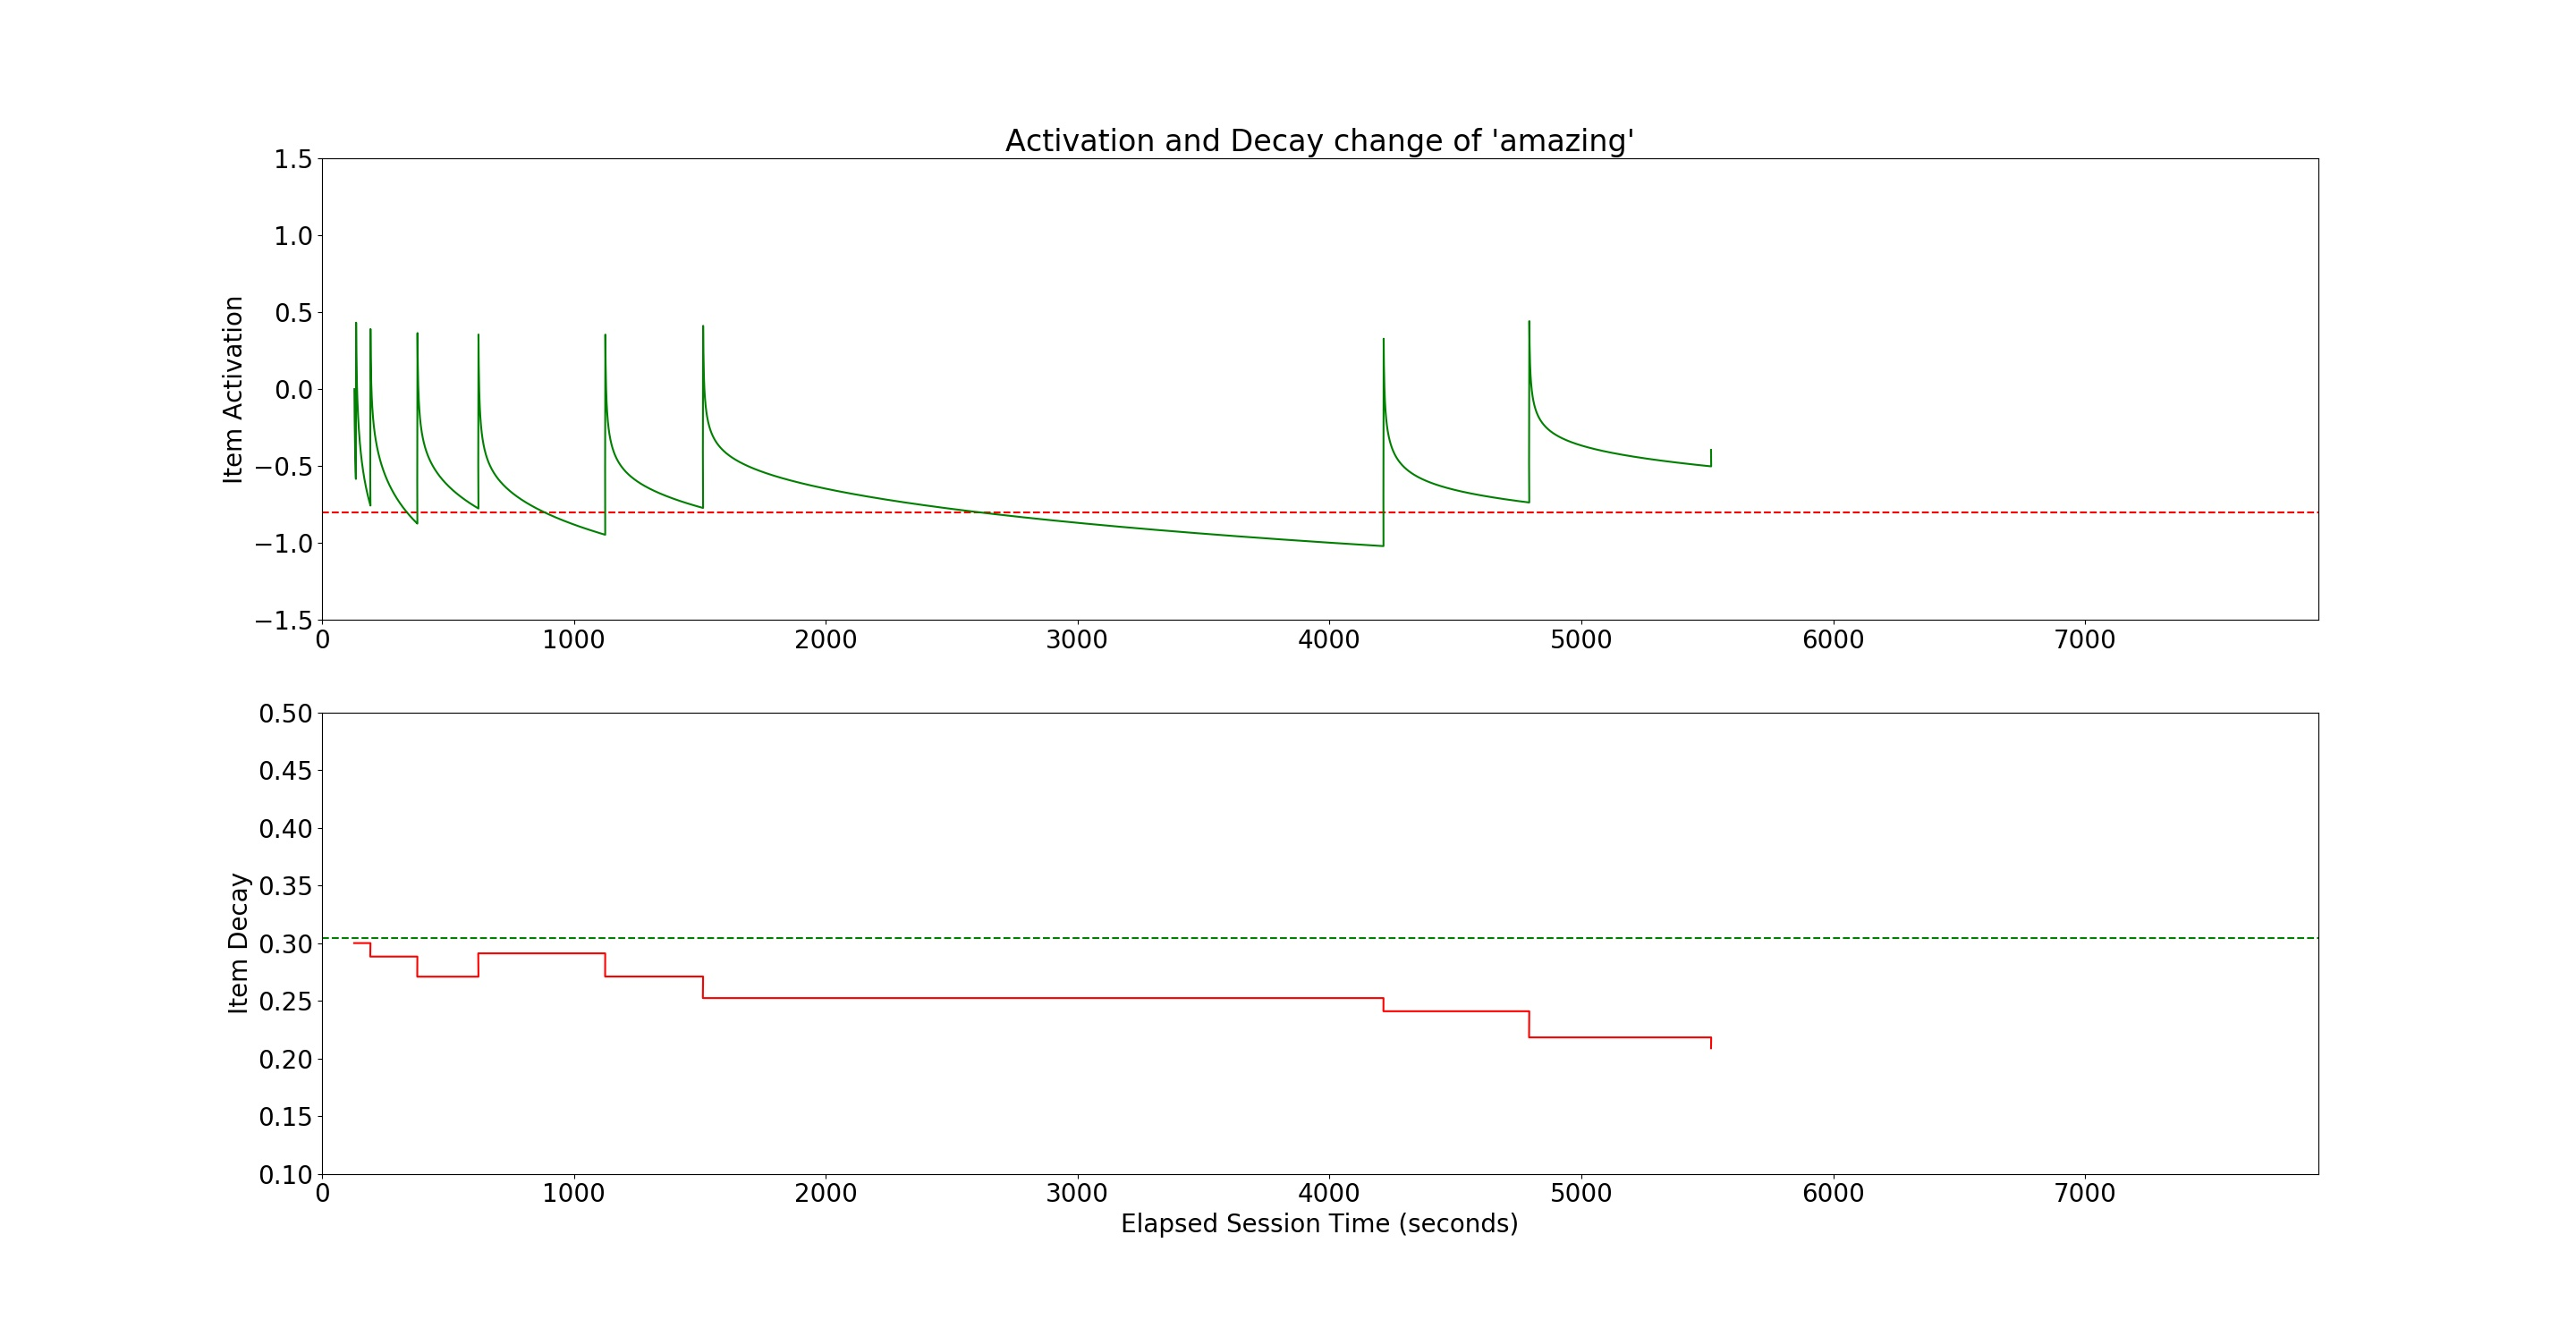
\includegraphics[width=12cm]{graph_activation.jpg}
\caption{Activation and decay change of the item "amazing" from a simulation of 2 study sessions, taking place 24 hours apart and lasting 30 minutes each}
\label{graph_act}
\end{figure}

\section{Enhancements of the Pavlik and Anderson Model}
The Pavlik and Anderson model has been used as a basis for a lot of the research which targets vocabulary learning (and factual learning in general). Extensions to the model have been made by \cite{pavlik07}; \cite{vans09}; \cite{nijboer11} and others. All of the proposed extensions keep the general idea of the model, but aim to improve the activation calculation to either better represent the learner or better show human learning and cognitive patterns.

In 2007 Pavlik suggested an improvement to the activation formula by adding 3 additional $\beta$ parameters (Formula \ref{eq:activation_ex}). Each of those parameters would contain either item-specific or learner-specific information, which would better represent the learner's connection to the particular item. Since different people learn at different rates, the $\beta_s$ parameter was added in order to introduce the learner's learning ability to the activation calculation. In addition to that, certain words are more difficult to learn than others (either because of their morphology or their semantics). To account for that, Pavlik added the $\beta_i$ parameter to the formula as well. The first two parameters are then combined in the $\beta_{s,i}$ parameter in order to represent the relative difficulty of a given item for the particular learner. To add an additional dimension to the calculation, the $b_j$ parameter was added, which allows the system to apply scaling to different word presentations. This means that it can now evaluate word-pair presentations differently than presentations of the word in context, which allows for much more control over the learning process. \citep{pavlik07}

\begin{equation}
\begin{large}
\label{eq:activation_ex}
m_i(t) = \beta_s + \beta_i + \beta_{s,i} + \ln{\Bigg(\sum_{j=1}^{n;t_j<t}{b_j(t - t_j)^{-d_{i,j}}}\Bigg)}
\end{large}
\end{equation}

Different approaches were taken by \cite{vans09} and \cite{nijboer11}. They proposed that the learner's reaction time be recorded and used when calculating the activation of each item. This suggestion is based on the idea that if the learner takes longer to finish the word encounter, then it is more difficult for them to recall the item from memory. Nijboer further expanded upon the idea of using reaction time by providing a way to predict the expected time needed to process the item presentation exercise (for example the time needed to read a sentence, before the learner has to attempt to retrieve a missing word from their memory).

\section{The problem}
Even though most of the proposed extensions have been shown to provide improved effectiveness of the model, none of them tackle the problem of computational efficiency. When integrated in a real-life system, an inefficient algorithm could inconvenience the user by making them wait while the activations of all items are calculated before each encounter, wasting precious learning time during the study sessions. Furthermore, since the activation calculation takes into account all previous encounters with the item, it becomes increasingly expensive when it comes to learning more difficult words (since they would require more encounters to learn). All of these factors have inspired this attempt at improving the computation time of the algorithm.

\section{Program optimization methods}
The process of program optimization usually aims to improve an algorithm by reducing the usage of a certain resource (whether it is execution time, hard drive space or another available resource). \citep{sedgewick11}. However, sometimes optimization with regards to one resource requires increased usage of another one. In the case of the Pavlik and Anderson learning algorithm, the valued resource is execution time (since the algorithm is executed before each item encounter and needs to quickly determine which word should be presented next).

Program optimization is usually applied using established and proven methods. Those methods differ in the level at which the optimization occurs, as well as in the type of optimization problem they are trying to solve. The different levels of program optimization include:
\begin{enumerate}
    \item Optimal choice of technologies
    \item Algorithm design with attention to resource efficiency
    \item Writing source code with attention to efficient command execution
    \item Compiler optimizations
\end{enumerate}

The higher levels of optimization (where most of the work is usually done by the developer instead of the computer) tend to have a greater impact on program efficiency than the lower ones. \citep{pottosin91}. This means that an inefficient algorithm, which was run on a highly optimized system will execute slower than an efficient algorithm, which was run on a sub-optimal system. Therefore the higher levels are usually targeted first when an optimization problem occurs.
    
Some of the most famous optimization methods make use of recursion in order to simplify the initial problem into smaller, more manageable sub-problems. One such method is the well known \textit{Divide and conquer}, which splits the initial problem recursively until the sub-problems are simple enough to be easily solved. \citep{smith85}. After the base problems are solved, their solutions are combined in a way that yields the solution to the initial problem. Divide and conquer algorithms have found a wide usage from sorting problems to syntactic analysis problems. \citep{algs_intro}

\subsection{Dynamic programming}
Another optimization technique, which tries to optimize recursively solvable problems is \textit{Dynamic programming}. While Divide and conquer is only suitable for problems, where the merging of the solutions to the recursively created sub-problems yields the result of the original problem, Dynamic programming is used in cases, where those solutions can be directly used to solve the original problem. The applicability of Dynamic programming techniques to the problem at hand depends on 2 properties: \textbf{optimal substructure} and \textbf{overlapping sub-problems}. Optimal substructure is fulfilled when an optimal solution to the problem contains optimal solutions to its sub-problems \footnote{notice that when talking about optimization, there is no single optimal solution, there are multiple possible ones}. The other property of Dynamic programming refers to the fact that problems, to which it is applied do not constantly generate new sub-problems at each step (which is what Divide and conquer algorithms tend to do), but instead repeatedly solve the same problems. Since this repeated solving is very inefficient, Dynamic programming promotes the use of \textit{Memoization} in order to store the results of sub-problems in a map so that the algorithm doesn't need to re-solve them every time they come up, but instead just fetch the solution from memory. \citep{algs_intro}

An example of a problem, to which Dynamic programming could be applied is generating a number from the Fibonacci sequence. This problem exhibits both optimal substructure (since each number is a result of summing all previous numbers) and overlapping sub-problems (calculating each number requires the calculating of all previous ones, which inevitably makes some of the calculations overlap). Other uses can be found in problems such as finding the shortest path, Levenstein distance calculation as well as parsing (The Earley chart parser). The activation calculation of Pavlik and Anderson's learning model, however, behaves in the same way that the Fibonacci sequence is calculated: in order to get the activation of an item at an encounter with a given time $t$, we need to calculate the activations of that item at all encounters, which occurred before the given one. Once the calculation recurses down, it causes a lot of the values to be recalculated, therefore using Dynamic programming techniques (in particular Memoization), could speed up the calculation and make it less demanding. Of course storing each word's activation for each encounter requires the usage of more hard drive space, but the size of this information should be small enough to justify the undeniable improvement in performance.

\subsection{Approximate computing}
Another approach to optimization can be observed in Approximate computing, which uses result accuracy as an available resource. This method is based on the idea that solving a problem, the accurate calculation of which proves to be quite resource-intensive, by instead approximating the result (within a limited range of error), provides an unexpected improvement in performance. Since result approximation can have catastrophic consequences if applied improperly, Approximate computing follows certain rules about which data can be approximated and which - not. The general rule states that only data which is not critical to the execution of the program can be approximated. Therefore it is up to the developer to carefully apply this method in order to achieve its potentially significant results. \citep{approx_computing}



\chapter{The Optimization Process}
\section{Naive implementation}
In its most inefficient form, Pavlik and Anderson's activation calculation algorithm is a mutual recursion between the activation function \ref{eq:activation_ex} and the decay function \ref{eq:decay}. The activation function depends on two sets of values: the timestamps of all encounters with a particular item and the item's decay rate at each of those encounters. While encounter timestamps are most likely already stored in each item's encounter history, calculating the decay proves a little bit more intricate. The item's decay intercept ($\alpha$) is easily accessible, but calculating the activation of the previous encounter requires multiple recursive calls between the two functions until no more previous encounters exist. Although this is inefficient, it should still function when the number of encounters isn't that big, but once an item has been encountered a certain number of times, the continuous mutually recursive calls overflow the stack \footnote{A stack overflow occurs when the capacity of a program's call stack is exceeded (i.e. there are too many function calls)}.

An obvious solution would be to simply store the activation value for each encounter (since a history of encounters is already being maintained) and then simply retrieve those activations whenever the decay rate needs to be calculated for a certain encounter. This, however, is further complicated due to the fact that the model adjusts based on the user's performance. As already mentioned, the model adjusts its representation of the user and their interaction with each item by tweaking the item's $\alpha$ value, which directly affects the item's decay rate and hence how frequently it is chosen for the next encounter. This results in the $\alpha$ value indirectly influencing the very activation of an item after each encounter. Since the activation value is constantly changing, retrieving it from memory at different times could produce invalid results.

\section{Base implementation}
In order to avoid the above scenario, it is more sensible to implement the algorithm in such a way, that recursion only occurs in the activation function. The purpose of recursing then is to calculate the activation of the previous encounter and once that is achieved, the value can be used for directly calculating the encounter's rate of decay. Although this solves the stack overflow problem, it is still a very inefficient solution with an exponential complexity. Since the activation function is recursively called $2^n$ times, where $n$ is the number of encounters in the item's encounter history, the algorithm will perform worse as the encounter histories of all items grow. \citep{sipser12}

A closer inspection of the learning algorithm shows that the bottleneck \citep{wescott13} occurs because of the number of function calls, which are executed with the same parameters. The reason for this is that calculating the activation of an item at the current encounter requires the activations of all previous encounters with the item to also be calculated. Recursing down, this results in the activations of earlier encounters being recalculated multiple times, because they are all (even though sometimes indirectly) needed for calculating the activations of latter encounters. For example if an item has only been encountered 3 times, calculating its activation at encounter 4 requires recursive calls to activations 3, 2 and 1, each of which also requires recursive calls to their previous encounters. In the end the activation of encounter 1 ends up being calculated 4 times and the whole process makes a total of 8 recursive function calls.

This behavior can also be observed when trying to generate a number from the Fibonacci sequence, since each number is the sum of all previous ones. Given that a more efficient implementation of the Fibonacci algorithm can be achieved by applying Dynamic programming techniques and that the activation algorithm fulfills both requirements for being able to use dynamic programming (the identical recursive calls prove that the activation algorithm includes overlapping sub-problems and the fact that each activation is dependent on all previous ones shows the optimal substructure of the algorithm), it is reasonable to attempt to apply dynamic programming to the activation calculation as well. This is achieved by caching the results of successfully executed recursive calls so that whenever the activation function needs to be executed with the same parameters, the result is simply retrieved from memory. Making use of this technique drastically decreases the time complexity of the algorithm from exponential to linear and speeds up the calculation. Instead of $2^n$ recursive calls (where $n$ is the number of times the item has been encountered), the algorithm now only makes $n+1$ calls (one for each previous encounter and one for the current one).

\section{Heuristic approach}
Despite the implementation described above significantly speeding up the calculation, the fact that this calculation occurs for each word before each item encounter and that it becomes more taxing as the number of encounters increases could require that it be further optimized in order to not hinder user interaction when faced with more difficult words or longer word lists. It is impossible to make further significant improvements to the time complexity of the actual activation calculation algorithm, but it is feasible to attempt to solve the problem with a heuristic approach. This would be based on reducing the amount of calculations done during the study session by making use of the time between sessions. There are two reasons why the recursive calculation needs to take place before each item encounter:
\begin{enumerate}
    \item The time, elapsed since the last encounter of each item affects the item's current activation
    \item The $\alpha$ value of each item is adjusted after each encounter in order for the model to adapt to each learner
\end{enumerate}
Although the elapsed time cannot be neglected, since it represents the spacing effect, it might be possible to make use of the changes in the items' $\alpha$ values when further optimizing the algorithm. In his PhD Thesis, Florian Sense shows that an individual's rate of forgetting ($\alpha$) stays relatively stable over time. \citep{sense17}. This information, combined with the experience of Approximate computing, can be utilized to develop a heuristic solution for faster activation calculations.

As mentioned above, the values around which the heuristic solution is built are the items' rates of forgetting ($\alpha$). Since those values are adjusted based on the outcomes of each user interaction with each item and since it is impossible to predict the outcomes in advance, no true approximation of these values can be made. Instead, this solution is based on caching the activation values of all previous encounters and then using the cached values whenever the current activation needs to be calculated, which results in each activation calculation requiring a single function call. Even though this means that the previous activations don't get recalculated with the newest $\alpha$, its stable rate of change should ensure that no substantial differences occur between the actual updated activation values and the cached ones. That being said, if the previous activations are never updated, they run the risk of becoming outdated once the difference between the current rate of decay and the one used for calculating a previous encounter's activation becomes significant enough. To prevent this from happening, the model should perform a complete update of the cached activations, which consists of recalculating the activations of all previous item encounters using the item's current $\alpha$ value. Since the goal is to avoid wasting time during study sessions, this update should take place between them, which preserves the user's interaction with the system during the actual process of studying.



\chapter{Evaluation of Performance (Setup and Results)}
All experiments conducted in order to research the spacing effect in vocabulary learning systems use varying parameters for their learning model (study session duration, time between study sessions, vocabulary size, etc.). The reason for this is because learner performance largely differs based on internal factors, such as the learner's language learning capabilities, their familiarity with the domain, in which particular words are used and others. This makes coming up with the perfect set of parameters a challenge. \citep{woudenberg08}. In order to provide a stable environment, which allows for comparison between the results of the different experiments, we have chosen to conduct simulations based on those in Christopher Dilley's Paper on the "Application of Personalized Adaptive Learner Modeling to Vocabulary Learning Software". \citep{dilley17}

\section{Simulation setup}
The experiments simulate a learning process, which consists of 2 study sessions, each lasting 30 minutes and taking place 24 hours apart. These values should allow for testing of the spacing effect not only during study sessions, but also in the time between them. The goal of the simulations is to replicate the process of a human learner being presented with a list of 37 words during the specified studying time.

The simulation system keeps track of two sets of $\alpha$ values for each word:
\begin{itemize}
    \item Real $\alpha$: randomly assigned to each word before the simulation in order to show how difficult that word is to learn
    \item Predicted $\alpha$: adjusted based on word interaction outcomes as a way of simulating the model's adaptability (starts at a default value of 0.3)
\end{itemize}
    
At each word encounter, a learner's response is simulated by calculating the probability of them being correct, which is based on the item's activation with respect to its \textbf{real} $\alpha$. This calculation can be seen in formula \ref{eq:recall_prob}, where:
\begin{itemize}
    \item $p_r$ is the probability that the given item will be recalled
    \item $m_i$ is the activation of the item at the current encounter
    \item $\tau$ is the forgetting threshold
    \item $s$ is a parameter used to smooth noise in the activation
\end{itemize}
\begin{equation}
\begin{large}
\label{eq:recall_prob}
p_r(m_i) = \frac{1}{1 + e^\frac{\tau - m_i}{s}}
\end{large}
\end{equation}
The probability is then used to simulate a loaded coin flip, which produces either a correct or an incorrect response. The formula is shown in \ref{eq:coin}, where $x$ is a randomly generated real number between $0.0$ and $1.0$. Depending on the simulated response, the model adjusts the \textbf{predicted} $\alpha$ in order to reflect whether the word is being learned. If the response was correct, the item's \textbf{predicted} $\alpha$ gets reduced by a certain amount, which results in a lower rate of decay for the item's activation and therefore causes the item to occur less often during study sessions. On the other hand, if the simulated response was incorrect, the \textbf{predicted} $\alpha$ is increased by a certain amount, increasing the item's activation decay and causing the item to be shown more often during studying.
\begin{equation}
\begin{large}
\label{eq:coin}
f(x) = 
\begin{cases}
    false, & \text{if } x < p_r\\
    true,  & \text{otherwise}
\end{cases}
\end{large}
\end{equation}

In certain cases the simulated item interaction produces a result, which only requires a slight adjustment of the predicted $\alpha$, which is reflected in formula \ref{eq:alpha_adjust}. In this formula:
\begin{itemize}
    \item $\alpha$(pred) is the $\alpha$ predicted by the model
    \item $p_r$(pred) is the recall probability, resulting from the predicted $\alpha$
    \item $0.02$ is the value chosen to adjust the $\alpha$
\end{itemize}
Producing expected results (a correct response when the recall probability is very high and an incorrect one when it is very low) means that the model already represents the learner's knowledge of the word correctly and therefore its $\alpha$ only needs a slight adjustment in order to include the outcome of the interaction. Producing the opposite outcomes (a correct answer when the recall probability is very low and an incorrect one when it is very high) means that the model's prediction of the item's alpha is incorrect and therefore needs to be adjusted more significantly in order to account for the user's progress or regress with respect to learning the particular item.
\begin{equation}
\begin{large}
\label{eq:alpha_adjust}
\alpha(pred) = 
\begin{cases}
    \alpha(pred) - (1 - (p_r(pred)) \times (2 \times 0.02))), & \text{if } success\\
    \alpha(pred) + (1 - (p_r(pred)) \times (2 \times 0.02))),  & \text{otherwise}
\end{cases}
\end{large}
\end{equation}

\section{Evaluation of performance}
In order to evaluate the progress of the algorithm optimization process, we tracked the duration of the simulations as a measure of how fast the activation computations took place and the average $\alpha$ errors as a measure of how accurately the model adapts to the user's performance.

Since the simulations do not require actual user interaction with the words, they track the duration of word encounters and study sessions by using an internal clock. This means that the most time during a simulation is spent on the process of calculating item activations when choosing the next item to be presented, which makes the duration a suitable measure of the calculation's performance. However, due to the use of random number generation when assigning the real $\alpha$s of each item, as well as when simulating the learner's response, we have taken the average duration of 50 simulations.

Keeping in mind that the model's goal is to adjust each item's predicted $\alpha$ based no the simulated learner interactions, the average $\alpha$ error (the average difference between each item's predicted $\alpha$ at the end of the simulation and its real one) can be considered a good measure of tracking the model's effectiveness in teaching words. Following the same logic as above, the average $\alpha$ error of 50 simulation was taken into account. This information not only allows comparison between the computational efficiency of the different algorithm implementations, but also reveals whether improvements in efficiency come at a cost of the algorithm's effectiveness.

\section{Result comparison (Cached recursion)}
The first performance comparison results can be observed below, in Table \ref{tab:cach_rec}. The displayed results are based on simulating learning using a vocabulary list of the size, specified in the first column and tracking the duration of the simulation. While the total number of encounters remains relatively stable regardless of the vocabulary size, we can see a positive correlation between the average number of encounters per word and the duration of the simulation. This occurs due to the fact that the increasing number of encounters in a word's encounter history slows down the activation computation, since the algorithm needs to recurse for every single encounter. The real performance comparison, however, is evident in the last two rows of the table, which both use a vocabulary size of 37 for the simulation. The difference between them is whether values were cached during the recursion of the algorithm in order to avoid recalculating of already computed data (described in Chapter 2, Section 3.2). As seen by the duration of the simulation, caching the values considerably speeds up the calculation and reduces the number of recursive calls that would be made during the $15^th$ encounter from 32768 to 16.

\begin{table}[h]
	\centering\small
	\scalebox{0.75}{
	\begin{tabular}{l*{6}{c}}
		\toprule
		& Item count & Encounter count & Encounter count & Function call count & Duration & Cached values \\
		& & (total, average) & (average per word) & (last encounter) & (simulation) & \\
		\midrule
		& 5   &   554 &   110.8   &  111   &  89.42s   & TRUE  \\
		& 10  &   559 &   55.9    &  57    &  45.35s   & TRUE  \\
		& 20  &   547 &   27.35   &  28    &  20.69s   & TRUE  \\
		& 37  &   560 &   15.135  &  16    &  12.61s   & TRUE  \\
		& 37  &   551 &   14.892  &  32768 &  2530.67s & FALSE \\
		\bottomrule
	\end{tabular}
	}
	\caption{Cached Recursion Test Results}
	\label{tab:cach_rec}
\end{table}

\section{Result comparison (Encounter duration)}
In order to accurately represent learner interaction and record the spacing effect, the simulation needs to advance its internal clock after each word encounter by an amount, resembling how much time an actual learner would take in order to complete the encounter. To achieve this, Formula \ref{eq:react_time}, which predicts the reaction time of the learner based on an item's activation, was used to calculate the amount of time it would take the learner to start interacting with the system after being exposed to the cue. \citep{vans09}. In this formula $F$ is a scaling factor for the reaction time, $f$ is the base reaction time and $m_{i,j}$ is the activation of item $i$ at a given encounter $j$.
\begin{equation}
\begin{large}
\label{eq:react_time}
RT_{i,j} =  
\begin{cases}
    3.788, & \text{if } m_{i,j} = -INF \\
    Fe^{-m_{i,j}} + f,  & \text{otherwise}
\end{cases}
\end{large}
\end{equation}
Since the learning process increases the reaction time, some padding was added in order to adjust the encounter duration to resemble that of a real life learner. The adjustment was based on the results, shown in Table \ref{tab:enc_dur}, which show that a too long or too short encounter duration do not accurately reflect the benefit of the spacing effect in the learning process. A padding of 3 seconds on top of the predicted reaction time was chosen, as it produced the most impressive combination of $\alpha$ error (difference between real $\alpha$ and predicted $\alpha$ at the end of the simulation), $\alpha$ bias (which of the two $\alpha$ values tends to be higher when calculating the error) and simulation duration compared to the rest of the tests.
\begin{table}[h]
	\centering\small
	\scalebox{0.9}{
	\begin{tabular}{l*{5}{c}}
		\toprule
		&  Padding  & Simulation duration & Encounter count  & Alpha error & Alpha error bias  \\
        & (seconds) & (seconds, average)  & (total, average) & (average)   & (average)   \\
		\midrule
		 & 0.5      & 35.34021312      &     1860.54      &  0.03527160 & -0.00513339 \\
		 & 1.0      & 17.28412206      &     1373.08      &  0.03351216 & -0.00488028 \\
		 & 1.5      & 11.35507244      &     1097.92      &  0.03301070 & -0.00329461 \\
		 & 2.0      & 6.381862320      &      918.52      &  0.03140569 & -0.00241167 \\
		 & 2.5      & 4.796245000      &      792.76      &  0.03173698 & -0.00071015 \\
		 & 3.0      & 4.051432420      &      697.50      &  0.03106919 & -0.00097124 \\
		 & 3.5      & 3.133872360      &      624.24      &  0.03159645 & -0.00054740 \\
		 & 4.0      & 2.568388580      &      566.64      &  0.03229276 &  0.00077986 \\
		 & 4.5      & 2.121258580      &      518.34      &  0.03333832 &  0.00166486 \\
		 & 5.0      & 1.874361840      &      478.92      &  0.03299457 &  0.00270733 \\
		 & 5.5      & 1.764593420      &      444.54      &  0.03491841 &  0.00289049 \\
		 & 6.0      & 1.561120180      &      416.44      &  0.03496761 &  0.00265287 \\
		 & 6.5      & 1.360384920      &      392.02      &  0.03649705 &  0.00458655 \\
		\bottomrule
	\end{tabular}
	}
	\caption{Encounter Duration Test Results}
	\label{tab:enc_dur}
\end{table}


\section{Result comparison ($\alpha$ adjustment value)}
Another important aspect of the model is how it adjusts the item $\alpha$s after each encounter. While some implementations of a spacing effect system use the learner's reaction time in order to calculate an appropriate new value (\cite{vans09}, \cite{koelewijn10}, \cite{nijboer11}, \cite{thiel10}), our implementation uses the item's recall probability as a way of scaling the adjustment value and applying it to the item's $\alpha$ depending on the outcome of the encounter. The $\alpha$ adjustment value is doubled, because of the fact that the model attempts to present words when they are at around 50\% recall probability (defined by the forgetting threshold $\tau$, which means that most of the time, the original adjustment value will be applied. The calculation can be seen in the formula \ref{eq:alpha_adjust}.
    
Tables \ref{tab:alpha_adjust_main} and \ref{tab:alpha_adjust_secondary} show that an $\alpha$ adjustment value of 0.02 not only leads to a lower average $\alpha$ error, but also provides stable results due to the fact that the $\alpha$ error is not skewed in favor of either the predicted $\alpha$ or the real one (expressed as Alpha error bias).

\begin{table}[h]
	\centering\small
	\scalebox{0.9}{
	\begin{tabular}{l*{6}{c}}
		\toprule
		 & Adjustment & Simulation duration & Encounter count  & Alpha error  & Alpha error bias  \\
         & (value)    & (seconds, average)  & (total, average) & (average)    & (average)   \\
		\midrule
		 &     0.02         & 3.92598758          &      698.68      &  0.035044720 & -0.00472192 \\
		 &     0.04         & 4.45247410          &      702.02      &  0.039973121 &  0.00621806 \\
		 &     0.06         & 4.86823896          &      708.12      &  0.048540735 &  0.01590292 \\
		 &     0.08         & 4.88345254          &      714.44      &  0.059730479 &  0.02860231 \\
		 &     0.10         & 4.68681396          &      720.22      &  0.073491184 &  0.04398006 \\
		\bottomrule
	\end{tabular}
	}
	\caption{Main Alpha Adjustment Value Test Results}
	\label{tab:alpha_adjust_main}
\end{table}

\begin{table}[h]
	\centering\small
	\scalebox{0.9}{
	\begin{tabular}{l*{6}{c}}
		\toprule
		 & Adjustment & Simulation duration & Encounter count  & Alpha error & Alpha error bias  \\
         & (value)    & (seconds, average)  & (total, average) & (average)   & (average)   \\
		\midrule
		 &     0.01   & 3.54518940          &      699.08      &  0.02890271 & -0.00337387 \\
		 &     0.02   & 4.43280080          &      696.82      &  0.02996629 &  0.00067759 \\
		 &     0.03   & 3.89115106          &      698.04      &  0.03399767 &  0.00552154 \\
		\bottomrule
	\end{tabular}
	}
	\caption{Secondary Alpha Adjustment Value Test Results}
	\label{tab:alpha_adjust_secondary}
\end{table}

\section{Result comparison (Cached encounter histories)}
The results of the implementation of the heuristic approach described in Chapter 3, Section 3.3 can be seen in Table \ref{tab:cach_hist}. The displayed data can be used to compare the performance of the algorithm when the activations of previous item encounters are cached and then used for calculating the activation of the current encounter and when they are not. The results additionally show how the algorithm performs when the cache is updated at various intervals. The first thing to note is that caching the item activations not only provides very similar results in terms of learning effectiveness (as evident by the similar $\alpha$ error values and biases), but also significantly improves the computational performance of the algorithm (proved by the impressively shorter simulation duration). The second important aspect of the results is the cache update interval. As already mentioned, even though caching all previous activations improves the algorithm's computational efficiency, if the cache is never updated, there will come a point where the items' $\alpha$s have been updated enough times for the data in the cache to become outdated and therefore lead to disastrous results. The fact that this claim is not supported by the data could be a result of each word in the given simulation having an average of 18 encounters and that possibly not being enough time for the cache to get outdated.

Keeping in mind that only one item's $\alpha$ changes after each item interaction, it would be reasonable to update the cache after each encounter (since only one item's activation would need to be recalculated). Table \ref{tab:cach_hist}, however, also shows that updating the cache after every encounter provides higher $\alpha$ error and is not as effective at improving the algorithm's performance. The most effective implementation is the one where the cache only gets updated after the study session is over. This helps avoid any unwanted fluctuations in the $\alpha$s during the sessions and does not allow for the cache to become out of date. The added benefit of this implementation is that since the cache update happens between study sessions, this does not influence the system's performance while it is in use and does not hinder user interaction.
\begin{table}[h]
	\centering\small
	\scalebox{0.75}{
	\begin{tabular}{l*{7}{c}}
		\toprule
		 & Encounter history & Cache update & Simulation duration & Encounter count  & Alpha error & Alpha bias  \\
         & (cached?)         & (when)       & (seconds, average)  & (total, average) & (average)   & (average)   \\
		\midrule
         & FALSE             &  -           & 22.5245806          &     697.94       & 0.03816317  & -0.01081656 \\
         & TRUE              &  -           & 4.10533710          &     700.34       & 0.03788089  & -0.01028201 \\
         & TRUE              & immediately  & 5.28907236          &     697.54       & 0.03825728  & -0.01085931 \\
         & TRUE              & post-session & 4.40695388          &     700.12       & 0.03764329  & -0.00930992 \\
		\bottomrule
	\end{tabular}
	}
	\caption{Cached Encounter History Test Results}
	\label{tab:cach_hist}
\end{table}

A more detailed overview of the simulation results with the finally optimized version of the Pavlik and Anderson learning algorithm (last row from Table \ref{tab:cach_hist}) can be seen in Appendix \ref{app:per_word_results}.

\section{Result comparison (Learning duration)}
As already mentioned, finding the most fitting combination of model parameters is highly dependent on various factors, among which is user performance. Since simulations provide unbiased results, they are suitable for a comparison between different model settings. The results of this comparison can be seen in Appendix \ref{app:learn_dur_results}, sorted according to their $\alpha$ error.

Based on the data, the different parameters hierarchically influence the model's effectiveness. Since the model is based on the spacing effect, the most influential parameter is the inter-session time. Simulations with study sessions, which took place 24 hours apart are shown to consistently perform significantly better than all other simulations. An explanation for this could be the fact that less inter-session time means more time spent learning words, which introduces competitors in the learner's mind and can influence the items' activations in memory. Furthermore, the inter-session time is scaled down in order to accommodate the spacing effect, therefore it being too short could neglect the effect and therefore influence learning. The second pattern, which is observed is that simulations with a higher session count and medium session duration tend to show better results. This signifies that study sessions, which last less than 15 minutes are generally not suitable for learning, possibly due to the fact that the activations of the items being learned have not been strengthened enough in the learner's memory, which results in slower learning speed overall. On the other hand, having a single session which lasts around 60 minutes (an example of "cramming") also performs poorly due to the lack of spacing in the item encounters.


\chapter{Outlook}
This thesis has provided an implementation which significantly improves the computational efficiency of the Pavlik and Anderson activation calculation algorithm by taking a heuristic approach based on the stable rate of forgetting of human memory. The algorithm can further be optimized by taking into account other of its properties or by implementing it in a system, where real learner input can be received and then analyzed in an attempt to discover patterns in the way actual humans process words.

\section{Shortening the encounter history}
Activation calculation becomes more expensive as the encounter history of an item grows. While there is a finite number of encounters, which a learner has to undergo in order to learn a particular word, the growing number will eventually influence the calculation to a point when its duration will impact the learner's interaction with the system. The solution to this problem is outside the scope of this thesis, but a possible approach would be to take advantage of the fact that the activation algorithm is designed in such a way as to consider the last encounter as the most impactful one for an item's current activation. This implies that all encounters before the last one provide progressively less impact to the item's current activation. In this case it is possible to attempt to further optimize the algorithm by empirically determining at what point in an item's encounter history can the activations of previous encounters be disregarded as they bring an insignificant contribution to the current activation. Doing this would allow a system to only calculate each item's activation based on a subset of its encounter history, which would naturally relieve the computation.

\section{Analyzing real learner data}
Simulations like the ones described in this thesis allow for optimization and testing of the algorithm itself, but an alternative approach is to base algorithm improvements on results, gathered from real learners. If the algorithm is implemented into a real system, the analysis of the gathered data could lead to useful information regarding the nature of human learning. Analysis could focus on finding patterns in the changes of item activations or $\alpha$ values after each word encounter. If such patterns are discovered, a possible optimization would be to cluster items according to the identified patters, which would allow for recalculation of whole clusters instead of individual items. Another analysis could attempt to cluster items according to the domain, in which they are used and attempt to directly link this to the domains, in which the language learner has previous knowledge in. If it is proven that a learner's previous knowledge in a domain affects how fast they learn other words from that domain, a system could take advantage of this information by predicting the learner's performance based on their previous knowledge and therefore use the predicted data to make even more efficient decisions as to the order in which the items should be presented.


\chapter{Conclusion}
Researchers are faced not only with the difficulty of developing a conceptually complex enough theory to model human memory, but also one computationally efficient enough to provide a reasonable user experience and thus applicable in real life vocabulary learning systems. This thesis has proven that using estimated values is an adequate solution for achieving that. The resulting model still takes into account the impact of the spacing effect, which is evident by the results of the learning duration test in Appendix \ref{app:learn_dur_results} (i.e. simulations with less spacing between study sessions generally performed poorly). The proposed implementation also achieved its goal of improving the computational efficiency of the original algorithm without compromising its effectiveness in vocabulary learning, which is supported by the fact that the $\alpha$ error values of the final implementation are closely comparable to those of the original algorithm implementation.

Technology enables such simulations and attempts at developing a model based on expected results, but its limits regarding the inability to fully represent how humans process language are still evident. Implementing the model into a real vocabulary learning system and collecting authentic language learner data not only makes further optimization based on patterns in the data possible, but also allows for more effective and adaptable learning. Whether it is the learner's familiarity with the domain in which a word is used or even orthographic, semantic or syntactic similarities between items presented shortly after one another, determining what makes learning more difficult allows for more accurate adaptations in a real system.

Employing the above suggestions should result in a highly efficient, adaptable and effective vocabulary learning system, which can be used as a basis for further implementations in the domain of discrete fact learning.



\appendix

\chapter{Final implementation results}
\label{app:per_word_results}
This appendix contains the item-specific data, gathered by calculating the average of 50 simulations of the final optimized version of the Pavlik and Anderson learning algorithm. The implementation builds on the base formula for calculating item activations (Formula \ref{eq:activation}) by caching values during recursion (explained in Chapter 3, Section 3.2) and caching encounter activations during study sessions (explain in Chapter 3, Section 3.3).

\begin{table}[h]
	\centering\small
	\scalebox{0.9}{
	\begin{tabular}{l*{7}{c}}
		\toprule
		 & Word               & Encounter count & Incorrect answers     & Alpha      & Alpha       \\
         &                    & (average)       & (percentage, average) & (real)     & (predicted) \\
		\midrule
         & noodles            & 17.54           & 33.47983264           & 0.29524848 & 0.28785772  \\
         & where              & 22.96           & 36.26889073           & 0.35149911 & 0.33767255  \\
         & many               & 15.44           & 29.21323734           & 0.24795644 & 0.26511870  \\
         & way                & 17.82           & 32.56175455           & 0.28869968 & 0.29017707  \\
         & market             & 33.12           & 37.18038195           & 0.42841451 & 0.40526655  \\
         & castle             & 19.04           & 34.08035733           & 0.32131938 & 0.30306387  \\
         & group              & 21.4            & 35.35670417           & 0.33082526 & 0.32554260  \\
         & restaurant         & 17.96           & 32.67135221           & 0.29574122 & 0.29328144  \\
         & amazing            & 19.52           & 34.97322791           & 0.31363545 & 0.30958762  \\
         & to visit           & 50.3            & 38.24197179           & 0.51870467 & 0.48669001  \\
         & each               & 19.18           & 34.35055572           & 0.31023359 & 0.30852093  \\
         & tree               & 18.22           & 33.90481349           & 0.30720531 & 0.29492939  \\
         & British            & 26.12           & 37.23884195           & 0.38105765 & 0.36367329  \\
         & adult              & 23.82           & 36.50340957           & 0.36267934 & 0.34791179  \\
         & a day              & 14.88           & 29.16932621           & 0.24498433 & 0.25996955  \\
         & open(from...to...) & 16.94           & 31.84299664           & 0.28801516 & 0.28339746  \\
         & furniture          & 12.64           & 23.95922688           & 0.18546626 & 0.23111772  \\
         & a year             & 10.08           & 14.02387612           & 0.03424036 & 0.19294444  \\
         & open               & 15.58           & 29.20736362           & 0.25710831 & 0.26877816  \\
         & free time          & 12.22           & 22.34968919           & 0.17272323 & 0.22695964  \\
         & canal              & 17.4            & 32.16698476           & 0.28683849 & 0.28735417  \\
         & Chinese            & 28.74           & 36.48165684           & 0.40444202 & 0.38434795  \\
         & stall              & 12.56           & 23.52746893           & 0.18401725 & 0.23226656  \\
         & playing field      & 13.38           & 25.22488841           & 0.22296496 & 0.24180841  \\
         & fancy              & 19.24           & 33.89328576           & 0.33149602 & 0.30983942  \\
         & a week             & 11.86           & 20.81879231           & 0.17367400 & 0.22061395  \\
         & to enjoy           & 24.46           & 35.89117006           & 0.36953320 & 0.35528614  \\
         & best               & 14.84           & 27.72794243           & 0.25163889 & 0.26202301  \\
         & wonderful          & 14.68           & 28.20075039           & 0.25321099 & 0.26166396  \\
         & expensive          & 21.16           & 34.21212479           & 0.34806222 & 0.32847172  \\
         & to add             & 27.96           & 36.08667367           & 0.40421330 & 0.37882536  \\
         & boat               & 19.78           & 33.38146256           & 0.32701793 & 0.31475231  \\
         & to join in         & 13.64           & 25.63385620           & 0.22608814 & 0.24977690  \\
         & view               & 15.82           & 30.02128520           & 0.27546900 & 0.27597488  \\
         & canoeing           & 11.04           & 16.69089799           & 0.08890224 & 0.21017056  \\
         & flower             & 15.52           & 28.48940741           & 0.26727894 & 0.27134638  \\
         & area               & 13.26           & 24.31336016           & 0.21747901 & 0.24556921  \\
		\bottomrule
	\end{tabular}
	}
	\caption{Final Implementation Per-Word Results}
	\label{tab:final_impl}
\end{table}



\chapter{Session spacing test results}
\label{app:learn_dur_results}
This appendix shows the top and bottom 10 results of running a simulation with the specified parameters.
\begin{table}[h]
	\centering\small
	\scalebox{0.9}{
	\begin{tabular}{l*{7}{c}}
		\toprule
		& Inter-session & Study session & Study session    & Simulation duration & Alpha error & Alpha error bias \\
        & time (hours)  & (count)       & length (seconds) & (seconds, average)  & (average)   & (average)   \\
		\midrule
         & 24           &     4         &     1800         & 20.32074736         &  0.03436126 & -0.00907207 \\
         & 24           &     3         &     1800         & 9.931795420         &  0.03447829 & -0.00937304 \\
         & 24           &     4         &     2700         & 64.18474976         &  0.03485828 & -0.00964994 \\
         & 24           &     3         &     3600         & 65.12516570         &  0.03491870 & -0.01075798 \\
         & 24           &     4         &     3600         & 158.1656642         &  0.03492370 & -0.00973170 \\
         & 24           &     3         &     2700         & 29.77002738         &  0.03508249 & -0.01027251 \\
         & 2            &     4         &     3600         & 154.5556253         &  0.03573720 & -0.01166020 \\
         & 4            &     4         &     2700         & 66.22802800         &  0.03574672 & -0.01053655 \\
         & 24           &     2         &     3600         & 24.25220504         &  0.03580125 & -0.01164732 \\
         & 24           &     4         &     900          & 3.157394600         &  0.03613755 & -0.00557596 \\
		\multicolumn{7}{c}{ . . . } \\
         & 24           &     2         &     1800         & 4.025952640         &  0.03866311 & -0.01145634 \\
		\multicolumn{7}{c}{ . . . } \\
         & 4            &     1         &     2700         & 1.860178920         &  0.04535570 & -0.01242237 \\
         & 24           &     2         &     900          & 0.700354800         &  0.04807315 & -0.00750375 \\
         & 4            &     2         &     900          & 0.703479280         &  0.04852638 & -0.00962511 \\
         & 2            &     2         &     900          & 0.838126240         &  0.04892341 & -0.01206129 \\
         & 4            &     1         &     1800         & 0.725312080         &  0.04956804 & -0.01062272 \\
         & 2            &     1         &     1800         & 0.848957300         &  0.04974269 & -0.01239915 \\
         & 24           &     1         &     1800         & 0.790586820         &  0.05019760 & -0.01193468 \\
         & 24           &     1         &     900          & 0.182783100         &  0.06301916 & -0.00923081 \\
         & 4            &     1         &     900          & 0.167927080         &  0.06326311 & -0.01127533 \\
         & 2            &     1         &     900          & 0.165350120         &  0.06338653 & -0.00920847 \\
		\bottomrule
	\end{tabular}
	}
	\caption{Learning Duration Test Results}
	\label{tab:learn_dur}
\end{table}


\chapter{Predefined constants}
\label{app:constants}
This appendix contains all predefined constants mentioned in this thesis.
\begin{table}[h]
	\centering\small
	\begin{tabular}{c*{3}{l}}
		\toprule
		& Constant         & Value  & Meaning \\
		\midrule
		 & $\alpha_d$      &  0.3   & Default starting $\alpha$ for all items \\
		 & $c$             &  0.21  & Rate of decay scale factor \\
		 & $\tau$          & -0.8   & Forgetting threshold \\
		 & $s$             &  0.255 & Recall probability noise reduction factor \\
		 & $\delta$        &  0.025 & Inter-session time scale factor \\
		 & $F$             &  1     & Reaction time scale factor \\
		 & $f$             &  0.3   & Base reaction time \\
		\bottomrule
	\end{tabular}
	\caption{Learn Duration}
	\label{tab:learn-duration}
\end{table}



\bibliography{bibliography}


\end{document}